\chapter{Discussion and Extensions}
\label{chap:discussion}

\section{What the Implemented Connection Establishes}
The principal result is an implemented connection between a human-specified local task and an executable motion--force skill. The teaching representation supplies pose, loading, and timing together. The policy consumes observations and generates that same kind of sequence. The common executor and existing contact controller make the output actionable on the robot. E1 and E2 then examine the physical behavior rather than equating a valid network output with successful processing.

The primary E1 comparison establishes that this connection produces an executable local contact skill. Rules, replay, and the learned provider each complete contact, the required loaded traversal, and exit in all five planned runs. Their execution characteristics differ: T has a shorter mean completion time and smaller time dispersion than C, and C has greater mean excess-force exposure. E2 then shows a shorter operator-based completion interval for the force-observing configuration than for B, together with an incomplete release transition in A4. The two comparisons support an implemented skill and configuration-dependent behavior while giving the fixed alternatives their observed value.

The comparison also clarifies what an execution-level result can establish. A generated rise can be learned as part of the demonstrated temporal structure. A gate can recognize unloading, and an evaluator can confirm a displacement. None of those observations directly measures remaining defect depth. Maintaining that distinction allows the method to be described positively and precisely without assigning hidden process reasoning to the policy.

\section{When Rules and Replay Are Sufficient}
The nominal task is narrow: a specified region, a single demonstrated direction, a fixed setup, and an existing lower-level controller. Under those conditions, a prescribed strategy has a strong opportunity to work well. T reuses a full force-inclusive episode and its timing, making it a substantive alternative rather than a deliberately impoverished baseline. Its short completed intervals and low observed dispersion indicate that a stable demonstration can be valuable without policy learning.

R illustrates the same point from a process-recipe perspective. A finite rule can express approach, loading, traversal, and departure directly. Its longer interval reflects the constructed strategy and contact synchronization, not an intrinsic limitation that all rules must be slower. Different recipe engineering could change that tradeoff, but no unexecuted recipe is used to reinterpret the measured comparison.

Imitation learning is used here to represent the demonstrated temporal relationship between motion and target force as an observation-conditioned generator. The specified region alone does not determine that relationship, but rules and replay can also supply it. E1 consequently evaluates learning alongside those alternatives rather than treating it as a necessary condition for completing the fixed task. T's strong nominal baseline and C's executable sequence are compatible findings: they characterize different ways to supply the local strategy.

\section{Roles of Human Guidance and Relative Representation}
Human guidance resolves where the local operation is intended to occur. Teaching supplies an example of how movement and loading can be organized. These are complementary contributions of the operator. A spatial mask, mark, or origin cannot be treated as a complete polishing strategy, and a demonstrated strategy cannot silently substitute for a new region specification.

The relative representation supports this division by learning position around a stain center and explicitly handling the stain direction at the policy boundary. A single-direction local movement pattern is reused by aligning live XY and the policy image with the teaching direction, then inversely rotating the generated XY path and adding the live center. This is an implemented spatial-generalization mechanism, rather than a future proposal. It addresses placement and in-plane direction through task registration while leaving observation-conditioned motion--force generation to the learned policy.

Its scope follows from the transformed channels. Z, tool orientation, and force are not rotated, and image adaptation is an in-plane warp about the interaction ROI. Thus the mechanism transfers the planar movement pattern without claiming complete pose--wrench equivariance or arbitrary-view invariance. E1/E2 disable direction alignment and cannot establish its empirical rotation-transfer range. The implementation's existence and its unmeasured performance within those comparisons are separate conclusions.

The fixed image interaction ROI also has a specific function. It focuses part of the visual representation around the calibrated tool interaction area while retaining a global feature. It is not an explicit defect-state channel. The current experiments evaluate the resulting observation path as a whole; they do not isolate whether a mark's appearance, pose, or force carries most of the policy's decisions.

\section{What Force Output and Observation Contribute}
Target-force learning allows the reference sequence to express a changing load, including a departure from a constant recipe. Measured-force observation provides information about the interaction that occurred rather than the load merely requested. Their roles are conceptually distinct and are separated by the E2 contracts.

The E2 observations identify differences in the organization of contact and release. C's mean operator-based completed interval is \BCSeconds~s (\BCPercent\%) shorter than B's, with five completed attempts in each. This is a descriptive comparison of separately trained checkpoints, not the same weights tested with a channel switched off. A4 exposes an incomplete transition in the motion-only condition, but one interrupted attempt does not identify missing force output as the cause. The generated motion, external constant-force interface, mechanical state, and timing can all contribute.

The magnitude of force peaks also limits an uncomplicated advantage claim. C does not reduce the E2 mean peak below A, and it has greater E1 excess exposure than R and T. A lower whole-window force mean can follow from less time spent in contact. It is therefore inadequate to call that lower mean an improvement in force-control accuracy or surface finishing.

The force-frame convention is another practical boundary. The resolved teaching-to-base relation supports empirical common-axis analysis, while the evaluated training file and online adapter retain their actual numerical conventions. The force-conditioning path was not redefined for this thesis. Its present performance is an observation about that implementation; a future frame-consistent learning comparison would be a separate experiment. Similarly, the executor suppresses tangential force commands, so a nine-dimensional learned action should not be described as a physically demonstrated three-axis force-tracking capability.

\section{Procedural Completion and Surface Quality}
The contact procedure is a meaningful intermediate target for local polishing. A tool must establish contact, move through the relevant region under load, and leave the surface. E1 provides explicit observations for that sequence. E2 contributes an operator-based interpretation of task progression that preserves the interrupted attempt.

Surface quality adds a separate requirement. A completed traversal may remove too little, too much, or unevenly depending on the material, tool, abrasive, speed, and pressure distribution. Visible marks may respond differently from fine scratches in metal. Before/after snapshots with changing viewpoint and occlusion cannot supply calibrated depth or roughness. Consequently, the thesis's measured results concern local contact-task execution, with visible marking changes used qualitatively.

This separation does not make the application incidental. It identifies the part of a polishing workflow that the present system actually transfers: a spatially registered temporal skill and its execution through contact feedback. It also identifies what must be added before a process-quality claim becomes defensible. The missing quality evidence cannot be replaced by a model-derived heatmap or by lower force peaks alone.

\section{Execution-Derived Dose}
\label{chap:removal_estimation}
The repository includes an execution-derived heatmap recorder. It integrates a Preston-style force--speed product along the measured path and optionally spreads it over a nominal tool kernel. Its diagnostic quantity can be expressed as
\begin{equation}
 D(x,y)=\sum_k\kappa\,F_{n,k}\,v_k\,\Delta t_k\,
                 K_{\mathrm{tool}}(x-x_k,y-y_k),
 \label{eq:preston_spatial}
\end{equation}
where \((x_k,y_k)\) is the recorded path location, \(F_{n,k}\) the implementation's selected force component or projection, \(v_k\) its selected speed, \(\Delta t_k\) the observation duration, and \(K_{\mathrm{tool}}\) a spatial spreading kernel. Without a measured coefficient and tool-response calibration, \(\kappa\) defines relative scale and \(D\) has arbitrary units. Different recorder/extension versions also make different kernel and speed-model choices.

\begin{figure}[tbp]\centering
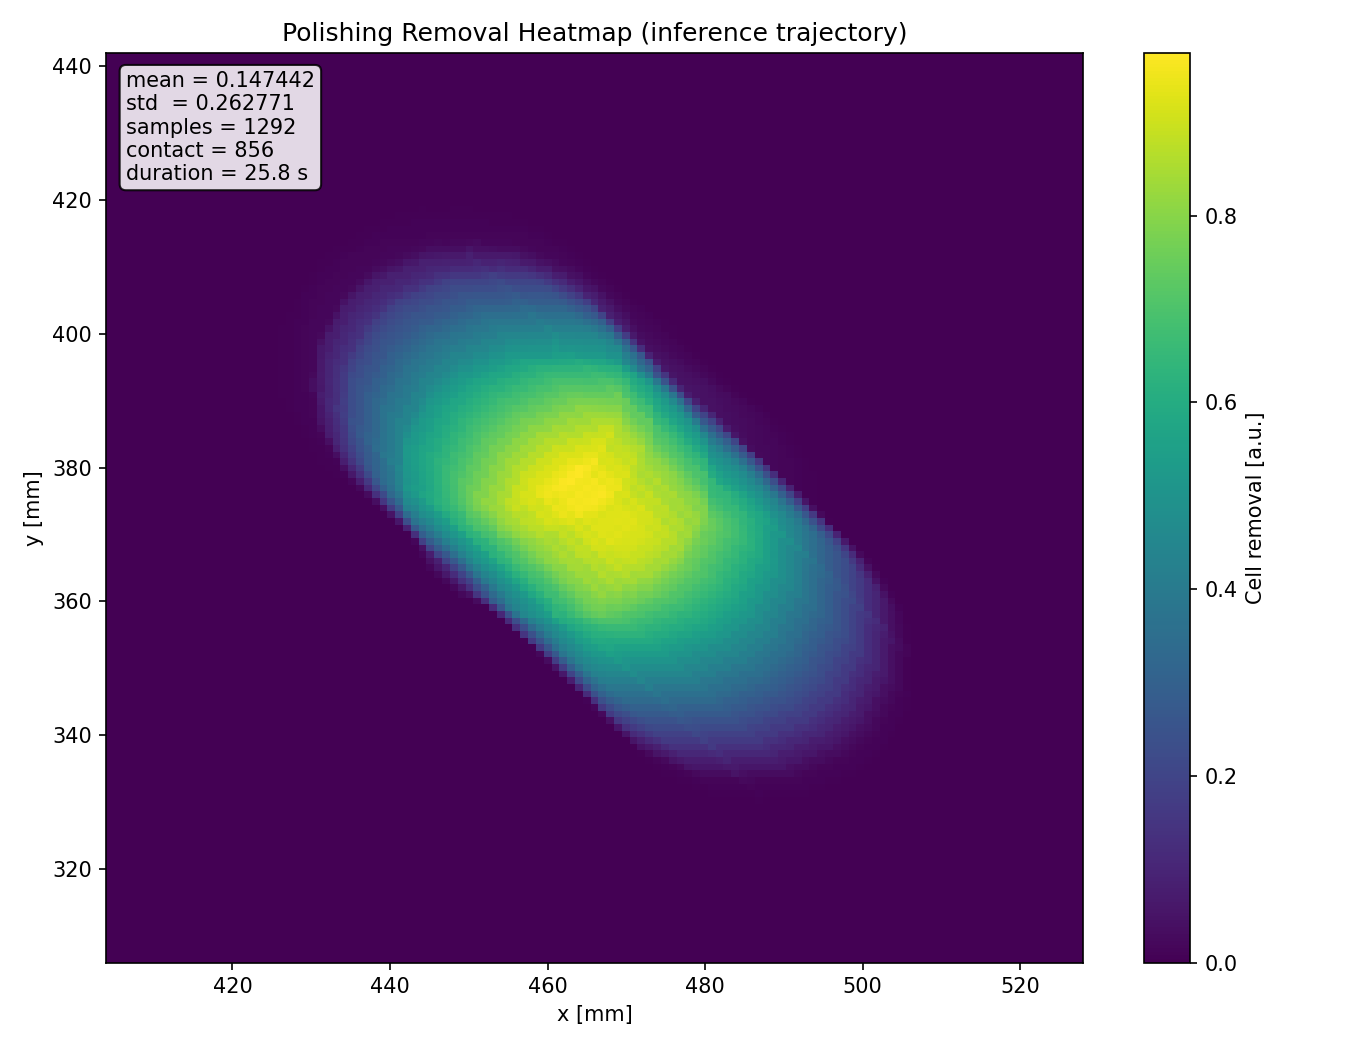
\includegraphics[width=\linewidth]{figures/E1_C1_diagnostic_heatmap.png}
\caption[Uncalibrated execution heatmap]{Historical execution-derived heatmap from E1 C1 on 14 October 2026, reproduced with its original axes and colorbar. Values are an uncalibrated model diagnostic in arbitrary units. They are not measured removal depth, effective contact footprint, or surface-quality improvement. This historical illustration is separate from the 15 October primary E1 cohort.}
\label{fig:diagnostic_heatmap}
\end{figure}

The implementation and generated artifact support calling this an implemented diagnostic extension. They do not support the older claim of a calibrated material-removal model. Its spatial distribution may help inspect where modeled processing exposure accumulated, but equal dose is not demonstrated equal removal on the actual specimen.

\section{Blending and Adaptive Execution Assets}
\label{chap:blending}
The project also contains finite local blending-path generation from an existing dose map, construction of an additional spatial target, and time allocation along a path. The 13 October extension prepares a sequence in which an initial skill is followed by a separate blending pass and diagnostic displays. Its archived validation includes offline planning from an earlier execution. That is evidence of an implemented extension, not an E1/E2 surface-uniformity result.

Separate 14 October adaptive-velocity records provide development experience with reference-clock progression and replanning. The located runtime files contain five online-OFF development attempts across multiple versions. Their completion status does not establish a controlled adaptive ON/OFF process-quality comparison. A later source revision addresses a recorded stalled reference-clock case, but its README explicitly distinguishes offline checking from a new physical run. These records are therefore kept outside the nominal E2 A/B/C cohort.

\begin{table}[tbp]\centering\small
\caption[Status of inherited extensions]{Status of inherited extensions relative to the main thesis evidence.}
\label{tab:extension_status}
\begin{tabularx}{\textwidth}{P{0.32\textwidth}X}
\toprule Asset & Supported status \\ \midrule
Execution heatmap & Implemented and generated from runs; uncalibrated arbitrary-unit diagnostic. \\
Finite blending planner & Implemented; archived offline planning and integration preparation. Surface-quality improvement not established by the main comparisons. \\
Adaptive reference-clock execution & Separate versioned development attempts and code; controlled ON/OFF outcome benefit not established. \\
High-level residual RL for curved-surface restoration & Planned extension; completed skill-level training and quality-grounded evaluation not established in the selected evidence. \\
\bottomrule
\end{tabularx}
\end{table}

An earlier thesis concept proposed residual adjustments to orientation and feed velocity based on residual removal demand. That concept remains a possible extension, with its old formulation retained in the preserved source. Existing low-level learned mass/damping control is a different asset and does not validate that proposed high-level policy. The core motion--force skill in this thesis does not require a removal estimator, blending planner, or residual RL stage to count as an executable system.

\section{Scope and Limitations}
The evaluation is confined to the fixed NOMINAL task. Physical height changes, reference Z offsets, new positions or directions, new shapes, and curved-surface performance are not evaluated. The direction-transfer adapter and inherited extension assets retain their implemented status, but are not experimental generalization results of E1/E2.

There is one trained checkpoint and one recorded training seed per learned condition, with five physical attempts per primary group. E1 shuffles methods within its five recorded blocks; E2 collects A, then B, then C. Neither the small groups nor the SDs establish statistical significance, equivalence, or population reliability. Reported dispersion concerns run-level time, peak force, and travel, not waveform reproduction or force-tracking accuracy. Setup preparation, tooling changes, and operator familiarity can remain alternative explanations for configuration differences.

The completion protocols also differ. E1 recognizes the first specified contact procedure using the recorded observer evidence. E2 includes the operator's observation and reaction, with possible lift and reapproach. Its \BCPercent\% B--C time difference therefore concerns that interval, not pure processing time or productivity at equal removal. A4's correction and C6's separate diagnostic role preserve the original observations without changing primary membership or removing unfavorable cases.

Surface depth, mass, roughness, and scratch-removal rate were not measured, so completion and visible marking changes support no quantitative surface-restoration claim. Likewise, an unrecorded controller-applied force target prevents a force-tracking-error claim. Future process-quality research can build on this execution framework, with those additional quantities treated as distinct scientific outcomes.
